\documentclass{standalone}
\usepackage[utf8]{inputenc}
\usepackage{tikz}
\usepackage{color}
\usetikzlibrary{arrows,shapes,positioning,shadows,trees}

\tikzset{
  basic/.style  = {draw, text width=3cm, drop shadow, font=\sffamily, rectangle},
  root/.style   = {basic, rounded corners=2pt, thin, align=center,
                   fill=yellow!60},
  level 2/.style = {basic, rounded corners=6pt, thin,align=center, fill=yellow!40,
                   text width=15em},
  level 3/.style = {basic, thin, align=left, fill=yellow!20, text width=8em}
}

\begin{document}

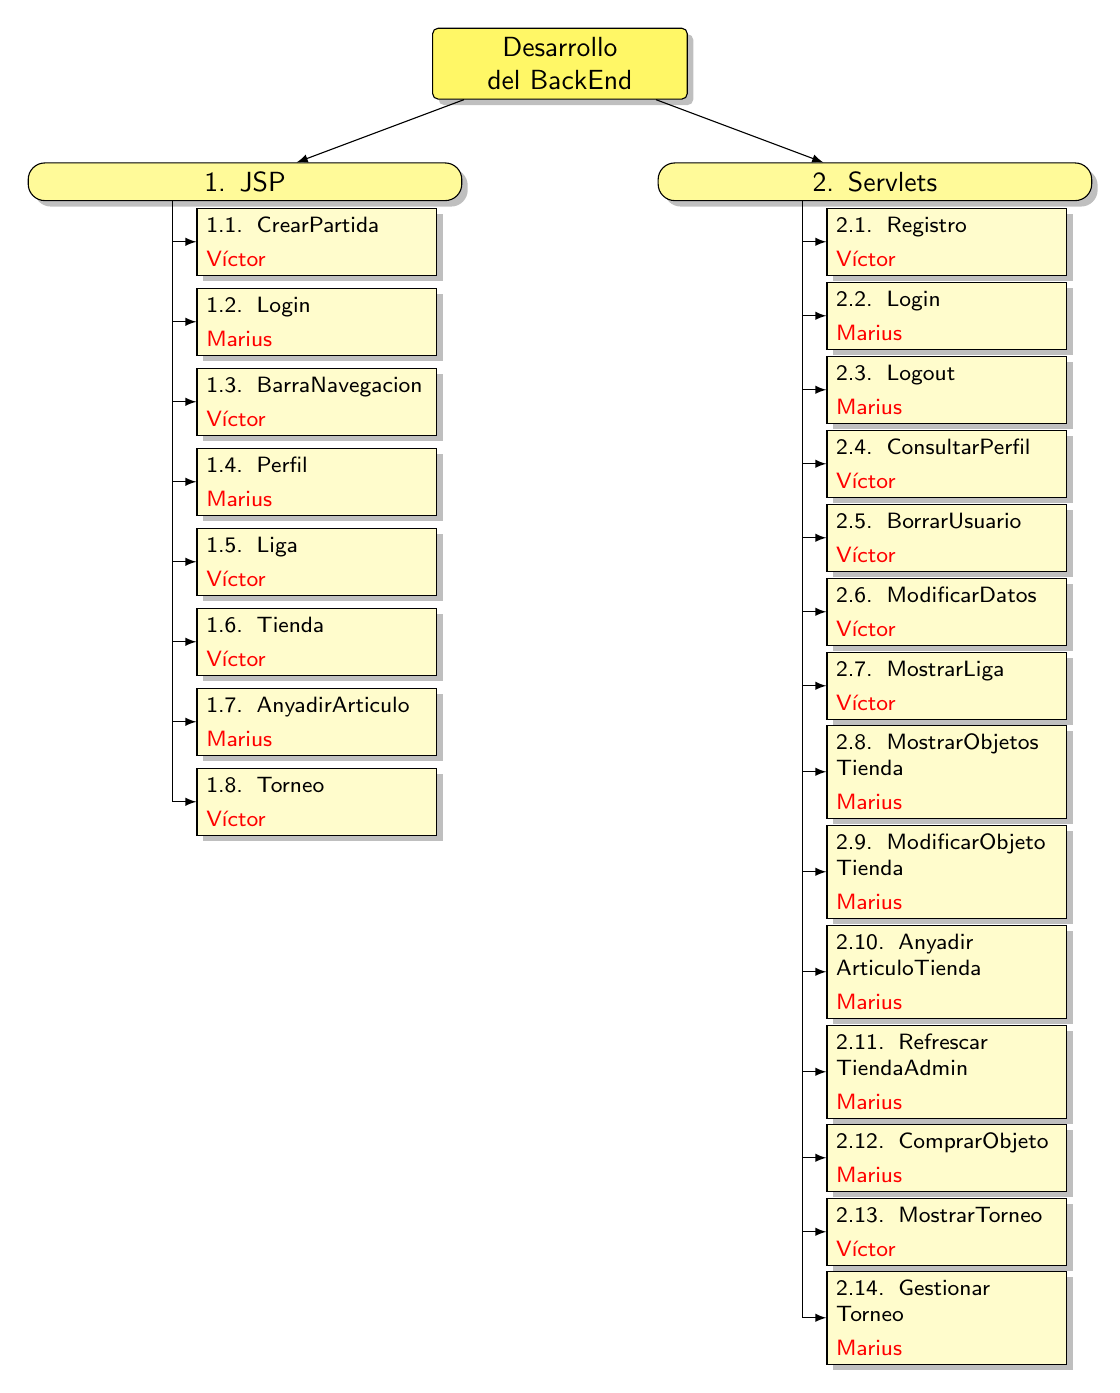
\begin{tikzpicture}[
  level 1/.style={sibling distance=80mm},
  edge from parent/.style={->,draw},
  >=latex]

% raiz inicial
\node[root] {Desarrollo del BackEnd}
% The first level, as children of the initial tree
  child {node[level 2] (c1) {1. JSP}}
  child {node[level 2] (c2) {2. Servlets}};

% The second level, relatively positioned nodes
\begin{scope}[every node/.style={level 3}]
\node [below of = c1,node distance=0.3in, xshift=26pt] (c11) {\footnotesize{1.1. CrearPartida} \\ \textcolor{red}{\footnotesize{Víctor}}};
\node [below of = c11,node distance=0.4in] (c12) {\footnotesize{1.2. Login} \\ \textcolor{red}{\footnotesize{Marius}}};
\node [below of = c12,node distance=0.4in] (c13) {\footnotesize{1.3. BarraNavegacion} \\ \textcolor{red}{\footnotesize{Víctor}}};
\node [below of = c13,node distance=0.4in] (c14) {\footnotesize{1.4. Perfil} \\ \textcolor{red}{\footnotesize{Marius}}};
\node [below of = c14,node distance=0.4in] (c15) {\footnotesize{1.5. Liga} \\ \textcolor{red}{\footnotesize{Víctor}}};
\node [below of = c15,node distance=0.4in] (c16) {\footnotesize{1.6. Tienda} \\ \textcolor{red}{\footnotesize{Víctor}}};
\node [below of = c16,node distance=0.4in] (c17) {\footnotesize{1.7. AnyadirArticulo} \\ \textcolor{red}{\footnotesize{Marius}}};
\node [below of = c17,node distance=0.4in] (c18) {\footnotesize{1.8. Torneo} \\ \textcolor{red}{\footnotesize{Víctor}}};

\node [below of = c2, xshift=26pt, node distance = 0.3in] (c21) {\footnotesize{2.1. Registro}\\ \textcolor{red}{\footnotesize{Víctor}}};
\node [below of = c21, node distance=0.37in] (c22) {\footnotesize{2.2. Login}\\ \textcolor{red}{\footnotesize{Marius}}};
\node [below of = c22, node distance=0.37in] (c23) {\footnotesize{2.3. Logout}\\ \textcolor{red}{\footnotesize{Marius}}};
\node [below of = c23, node distance=0.37in] (c24) {\footnotesize{2.4. ConsultarPerfil}\\ \textcolor{red}{\footnotesize{Víctor}}};
\node [below of = c24, node distance=0.37in] (c25) {\footnotesize{2.5. BorrarUsuario}\\ \textcolor{red}{\footnotesize{Víctor}}};
\node [below of = c25, node distance=0.37in] (c26) {\footnotesize{2.6. ModificarDatos}\\ \textcolor{red}{\footnotesize{Víctor}}};
\node [below of = c26, node distance=0.37in] (c27) {\footnotesize{2.7. MostrarLiga}\\ \textcolor{red}{\footnotesize{Víctor}}};
\node [below of = c27, node distance=0.43in] (c28) {\footnotesize{2.8. MostrarObjetos\\Tienda}\\ \textcolor{red}{\footnotesize{Marius}}};
\node [below of = c28, node distance=0.5in] (c29) {\footnotesize{2.9. ModificarObjeto\\Tienda}\\ \textcolor{red}{\footnotesize{Marius}}};
\node [below of = c29, node distance=0.5in] (c210) {\footnotesize{2.10. Anyadir\\ArticuloTienda}\\ \textcolor{red}{\footnotesize{Marius}}};
\node [below of = c210, node distance=0.5in] (c211) {\footnotesize{2.11. Refrescar\\TiendaAdmin}\\ \textcolor{red}{\footnotesize{Marius}}};
\node [below of = c211, node distance=0.43in] (c212) {\footnotesize{2.12. ComprarObjeto}\\ \textcolor{red}{\footnotesize{Marius}}};
\node [below of = c212, node distance=0.37in] (c213) {\footnotesize{2.13. MostrarTorneo}\\ \textcolor{red}{\footnotesize{Víctor}}};
\node [below of = c213, node distance=0.43in] (c214) {\footnotesize{2.14. Gestionar\\Torneo}\\ \textcolor{red}{\footnotesize{Marius}}};
\end{scope}

\foreach \value in {1,...,8}
  \draw[->] (c1.195) |- (c1\value.west);
\foreach \value in {1,...,14}
  \draw[->] (c2.195) |- (c2\value.west);
\end{tikzpicture}

\end{document}
